\usepackage{graphicx} 
\usepackage{verbatim}
\usepackage{hyperref}
\hypersetup{
    colorlinks,%
    citecolor=black,%
    filecolor=black,%
    linkcolor=black,%
    urlcolor=blue
}

\graphicspath{{../figures/}}

\mode<article>{\usepackage{fullpage}}
\mode<presentation>{\usetheme{default}}

\newcommand{\ftitle}[1]{\frametitle<presentation>{#1}}
\newcommand{\cmd}[1]{\begin{quote}{\tt #1}\end{quote}}

\title{UNIX Workshop\\\url{http://www.comp.nus.edu.sg/~melvin/UWS/}}
\author{Chua Wei Hang, Lim Jing Quan, Max Tan, Melvin Zhang}

% Use a top down style, currently still rather bottom up

\AtBeginSection[]{
   \begin{frame}{Outline}
   \tableofcontents[currentsection]
   \end{frame}
}

\AtBeginSubsection[]{
   \begin{frame}{Outline}
   \tableofcontents[currentsubsection]
   \end{frame}
}

\begin{document}

\maketitle

\mode<presentation>{
  \begin{frame}
  \titlepage
  \end{frame}
}


\begin{frame}
\ftitle{Jurassic Park (1993)}
\begin{quote}
``It's a UNIX system! I know this.''
\end{quote}
\begin{flushright}
-- Alexis ``Lex'' Murphy, Jurassic Park (1993)
\end{flushright}
\end{frame}


\section{Introduction to UNIX}
\begin{frame}
\ftitle{Acknowledgement}
The materials for this workshop are adapted from the following sources:
\begin{itemize}
\item UNIX Workshop 2005 notes by Mark Tan (SoC, NUS)
\item CS1101 Lab 0 notes by Aaron Tan (SoC, NUS)
\item UNIX/Linux Tutorial for Beginners by Michael Stonebank (University of Surrey)
\end{itemize}
\end{frame}

% Explain motivation/purpose/objective of UNIX workshop
% briefly explain what is UNIX and its relevance to SoC, industry

As an SoC student, you have access to IT facilities exclusive to SoC. Most of
these facilities are accessed via our \texttt{sunfire} server which runs the
Solaris Operating System, a UNIX-like operating system.  

UNIX is the name of the operating system developed by a group of AT\&T
researchers at Bell Labs in 1969.  Solaris and many other modern operating
system, such as Linux, Mac OS X, and BSD, are descendants of UNIX. All of these
operating systems provide a UNIX-like environment to the user. 

% applications
% benefits and uses of UNIX account
\begin{frame}
\ftitle{UNIX in SoC}
The UNIX environment provided by the Solaris OS on our servers are used for:
\begin{itemize}
\item writing programs for your programming labs/assignments
\item learning about operating system concepts (CS2106, Operating Systems)
\item hosting a database driven site (CS2102, Database Systems)
\item accessing SoC printers and checking your print quota
\item reading your SoC email account
\end{itemize}
\end{frame}

\begin{frame}
\ftitle{What is an Operating System?}
\begin{figure}
\begin{center}
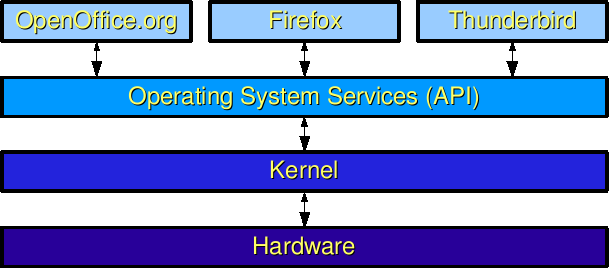
\includegraphics[width=0.7\linewidth]{os-layers}
\end{center}
\caption{Relation between applications, OS and hardware}
\label{fig:os}
\end{figure}
\end{frame}

An OS is the software that is in charge of scheduling resources and processes 
of a system as well as managing and maintaining interactivity between the
software and hardware of the system. Figure \ref{fig:os} shows that the
operating system acts as the bridge between your applications and the computer
hardware.  

\subsection{Origins of UNIX}
% people, time, place (story of invention)

\begin{frame}
\ftitle{Creators of UNIX}
\mode<presentation>{
\begin{figure}
\begin{center}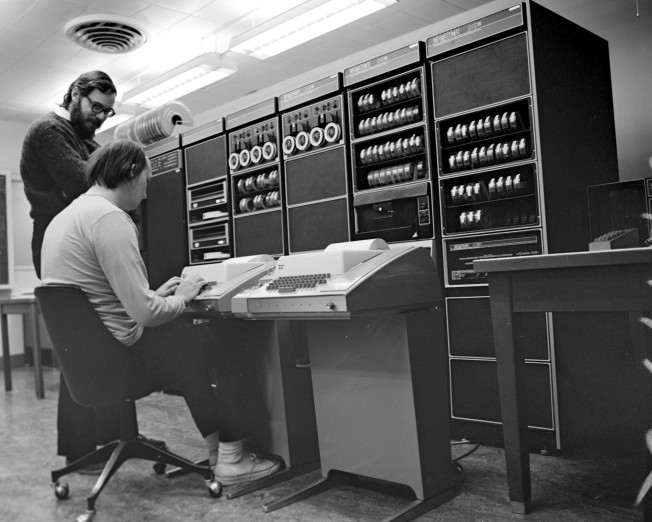
\includegraphics[width=0.7\linewidth]{dennis-ken2}\end{center}
\caption{Dennis Ritchie (standing) and Ken Thompson working on a
PDP-11.}
\end{figure}
}
\end{frame}

\begin{frame}
\ftitle{Creators of UNIX}
\begin{figure}
\begin{center}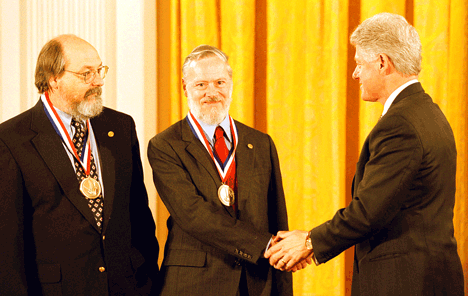
\includegraphics[width=0.7\linewidth]{dennis-ken3}\end{center}
\caption{Ken Thompson (left) and Dennis Ritchie receiving the National Medal of
Technology from President Clinton.}
\label{fig:medal}
\end{figure}
\end{frame}

The first version of UNIX was developed by Ken Thompson in August of 1969,
supposedly in just three week. In 1971, Dennis Ritchie invented the C
programming language and UNIX was rewritten using C and became the first
operating system to be written in a high level language. Most operating systems
of the time, including the original UNIX, was written in assembly language,
which was a special language that is unique to a particular type of hardware.
After UNIX was rewritten in C, it was possible to run UNIX on many different
types of hardware.     

For the development and implementation of UNIX and their contributions to
operating systems theory, Dennis and Ken were jointly awarded the A. M. Turing
award in 1983 and the National Medal of Technology (Figure \ref{fig:medal}) in
1999. The A. M. Turing award is the equivalent of the Nobel prize in Computer
Science.  

\begin{frame}
\ftitle{UNIX Family Tree}
\begin{figure}
\begin{center}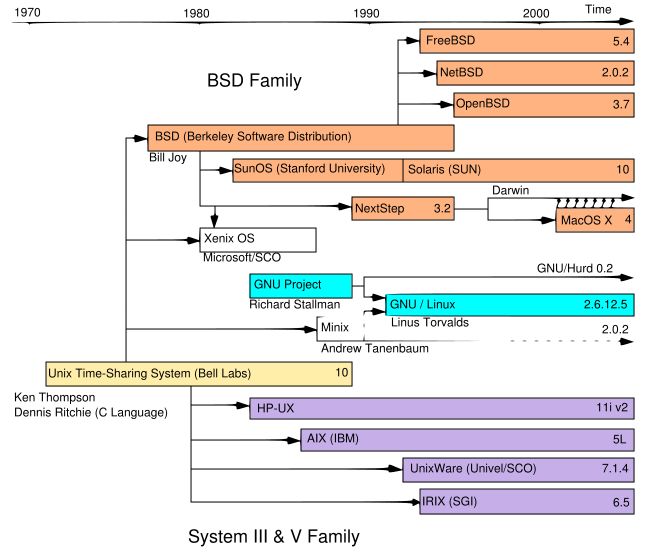
\includegraphics[width=0.7\linewidth]{unix_timeline}\end{center}
\caption{UNIX and its descendants}
\label{fig:timeline}
\end{figure}
\end{frame}

% UNIX in the modern context, Mac OS X, Linux
Today, many of the operating system, such as the Mac OS X from Apple, Solaris
from Sun and Linux, are descendants of the original UNIX system from Bell Labs
(see Figure \ref{fig:timeline}). The operating system you will be using on our
UNIX server in SoC is the Solaris OS.

\subsection{UNIX Concepts}
UNIX consists of the following components:
\begin{description}
\item[Kernel] The kernel of UNIX is the core of the operating system. It
allocates time and memory to programs and handles the file system and
communications in response to system calls.  
\item[Shell] The shell acts as an interface between the user and the kernel.
When a user logs in, the login program checks the username and password, and
then starts another program called the shell.   The shell is a command line
interpreter. It interprets the commands the user types in and arranges for them
to be carried out. The commands are themselves programs: when they terminate,
the shell gives the user another prompt.  
\item[Files and processes] Everything in UNIX is either a file or a process.  A
process is an executing program identified by a unique process identifier.  A
file is a collection of data. They are created by users using text editors,
running compilers etc.
\item[Utilities] An operating system is useless without useful applications that
help the you to accomplish everyday tasks such as editing text, browsing the web
etc.  A UNIX-like environment provides a standard set of useful utilities.  
\end{description}

\section{UNIX in SoC}
% NUSNET and UNIX account in SoC

Every NUS student is provided with a NUSNET account which gives you access to
university wide online services such as the Integrated Virtual Learning
Environment (IVLE) and an email account with the nus.edu.sg domain. 

In order to login to the PCs in the computer labs, you will need to use your
NUSNET account.   

% ACTIVITY
\begin{frame}{Activity: Login to NUSNET}
\begin{enumerate}
\item Press \texttt{Ctrl-Alt-Delete}.
\mode<presentation>{
\begin{figure}
\begin{center}
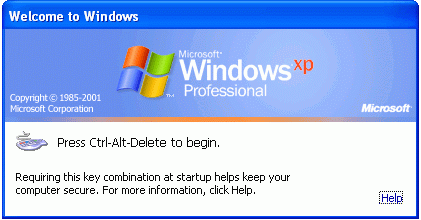
\includegraphics[scale=0.3]{ctrl_alt_delete}
\end{center}
\end{figure}
}
\item Type in your NUSNET username, password and select NUSSTU domain.  
\mode<presentation>{
\begin{figure}
\begin{center}
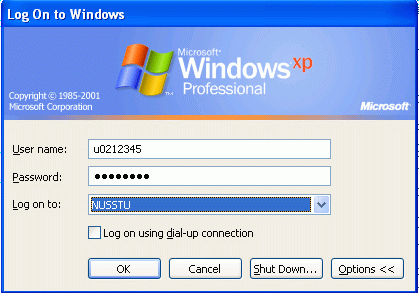
\includegraphics[scale=0.3]{stu_login}
\end{center}
\end{figure}
}
\item Click on the \texttt{Ok} button.  
\end{enumerate}
\end{frame}

In addition, every SoC student is provided with a UNIX account which gives you
access to SoC's \texttt{sunfire} server which run on Solaris. You are allowed to
choose your own username, for your UNIX account.  

In the following activity, you will create your UNIX account.  

% ACTIVITY
\begin{frame}{Activity: Creating your UNIX account}
\begin{enumerate}
\item Login to \url{https://mysoc.nus.edu.sg/~newacct} using your NUSNET
username and password.  
\item Read through the user-agreement and make sure you understand the
obligations. 
\item Decide your UNIX username.  Your username should be between 5-8 characters and
must be formed from your name.  You may also use your NUSNET username. 
\item Type in your new password (twice).
\item Submit your application.
\end{enumerate}
\end{frame}

\begin{frame}
\ftitle{Privileges}
Your new UNIX account comes with the following privileges:
\begin{itemize}
\item Email : \texttt{unix\_username@comp.nus.edu.sg}
\item Website : \url{http://www.comp.nus.edu.sg/~unix_username}
\item Solaris zone: \url{unix_username-z.comp.nus.edu.sg}
\item Disk quota: 2Gb
\item Print quota: 50 pages/month
\end{itemize}
\end{frame}

\subsection{Checking your SoC email account}
\begin{frame}
\ftitle{Checking UNIX email}
% Checking UNIX email, show webmail version, refer to CF site for details on
% setting up mail client, email forwarding from MySoC
You can access your UNIX email account via mySoC Webmail, \url{http://mysoc.nus.edu.sg/~webmail}
\mode<presentation>{
\begin{figure}
\begin{center}
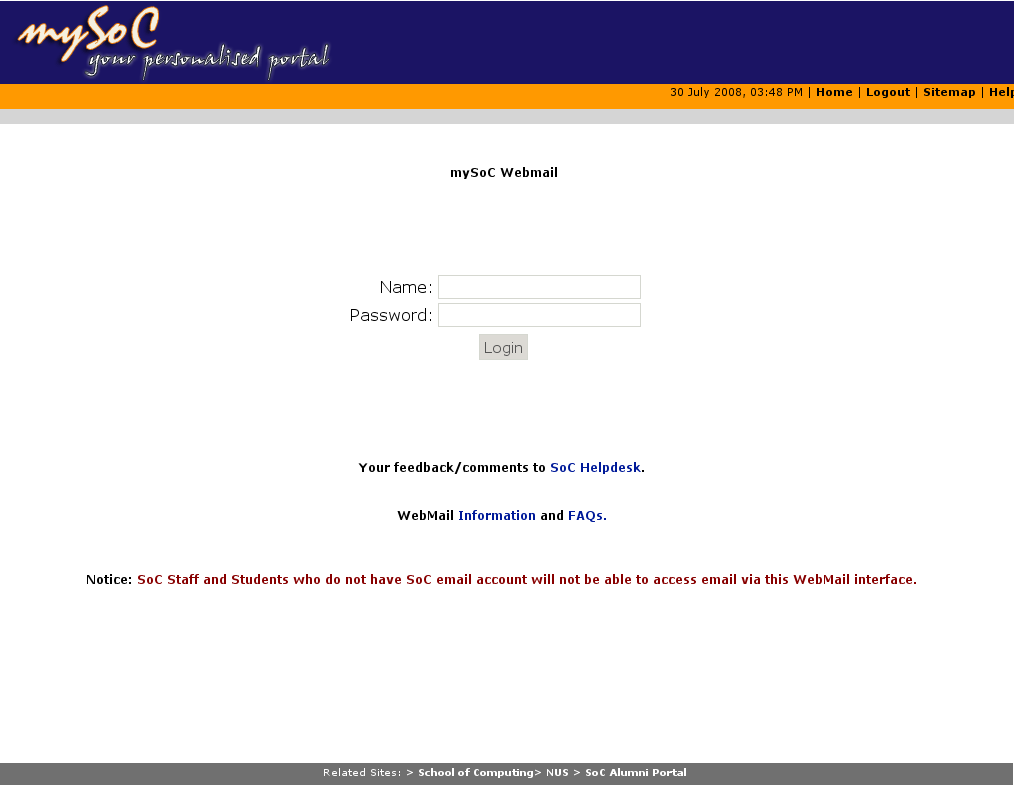
\includegraphics[scale=0.15]{mysoc_webmail}
\caption{mySoC Webmail interface}
\end{center}
\end{figure}
}
Your mailbox part of your disk usage, which is 2Gb. You can forward your NUSNET
email to your UNIX email using \url{https://exchange.nus.edu.sg/autoforward}.
\end{frame}

\subsection{SoC's \texttt{sunfire} server}
\begin{frame}
\ftitle{\texttt{sunfire} server in the Machine Room}
\begin{figure}
\begin{center}
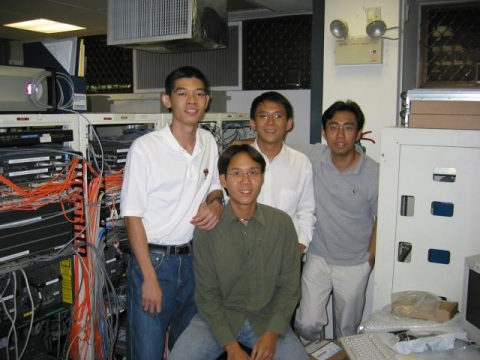
\includegraphics[scale=0.5]{machine_room}
\caption{\texttt{sunfire} server located in the Machine Room with our Networks
staff. Clockwise from top-left: Tan Chee Sin, Tan Kwang Pon, Budiman Tsjin
(has since left SOC) and Lai Zit Seng.}
\label{fig:sunfire}
\end{center}
\end{figure}
\end{frame}

In the next activity, we will connect to the \texttt{sunfire} server (see Figure
\ref{fig:sunfire}) and access the UNIX system via the Secure Shell protocol
(ssh).

\begin{frame}{Activity: Connecting to \texttt{sunfire}}
\begin{enumerate}
\item From the desktop, launch the \texttt{SSH Secure Shell Client} application. 
\item Click on \texttt{Quick Connect}\\ 
Host Name: \texttt{sunfire.comp.nus.edu.sg}\\ 
User Name: your UNIX username
\mode<presentation>{
\begin{figure}
\begin{center}
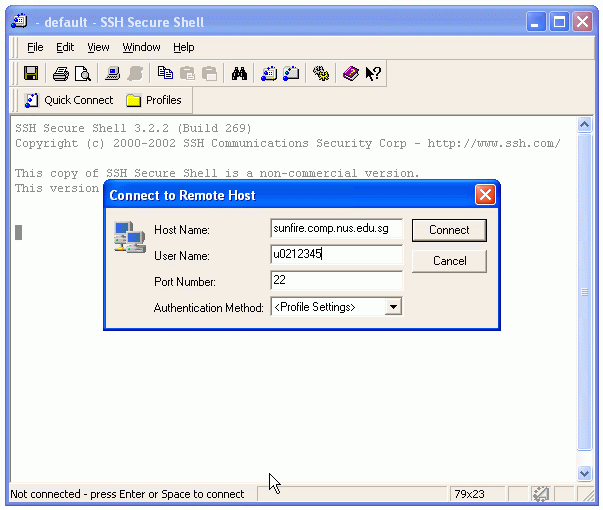
\includegraphics[scale=0.25]{ssh_sunfire}
\end{center}
\end{figure}
}
\item Click on \texttt{Connect}. Enter your UNIX password in the password dialog.  
\end{enumerate}
\end{frame}

Once you have logged in, a copy of the shell is started and you are
automatically placed in your home directory.  

The shell is based on a command line interface (CLI), this is in contrast to the
more commonly seen graphical user interface (GUI) which you are familiar with.
Both types of interfaces are useful, depending on the kind of activity.  

% CLI
% + power of piping and redirection, greater control
% + portable (available in many systems)
% + least overhead
% + easy remote access
% + faster to get things done
% + can be easily automated/scripted
% - higher learning curve
% - not easy to multi-task

% GUI
% + display of dynamically modifiable information
% + aesthetics
% + media
% + true multitasking
% + more intuitive, easier to learn

%* You can do things very quickly on command line.
%* GUI prevents you from understanding and learning the functionality happening behind the scenes.
%* Repetitive things can be automated easily using command line.

% GUI: WYSIWYG = WYSIAYG
% CLI: suited to performing ad hoc operations, to quickly combine a few commands
% to perform a query or some tasks

\begin{frame}
\ftitle{CLI vs GUI}
\begin{block}{Graphical User Interface}
What they tell you, WYSIWYG (What you see is what you get). \pause
The truth is, WYSIAYG (What you see is all you get).
\end{block}

\pause

\begin{block}{Command Line Interface}
\begin{itemize}
\item Suited to performing ad hoc operations by combining a few commands.  
\item Easy to automate repetitive tasks.
\item Default interface when accessing remote servers.  
\end{itemize}
\end{block}
\end{frame}


\subsection{Creating text files}
Types of files you will encounter on UNIX include the following:
\begin{itemize}
\item a document (report, essay etc.)
\item the text of a program written in some high-level programming language
\item instructions comprehensible directly to the machine and incomprehensible 
to a casual user, for example, a collection of binary digits (an executable or 
binary file)
\item a directory, containing information about its contents, which may be a 
mixture of other directories (subdirectories) and ordinary files.
\end{itemize}

% importance of good text editor
% on unix: vim, emacs, nano, pico 


Text files are used extensively on a UNIX system for storing system data,
program configuration files, scripts and source code. They are preferable to
binary files because they can be easily read/modified.  The most important
program is a text editor, a program to interactively create/edit text files.
Examples of editors on UNIX are Vim, Emacs, nano, and pico. 

\begin{frame}
\ftitle{Text files are ubiquitous on UNIX}
\mode<presentation>{
Program source code are stored as text files. A good text editor, such as Vim,
can dramatically improve your productivity.

\begin{figure}
\begin{center}
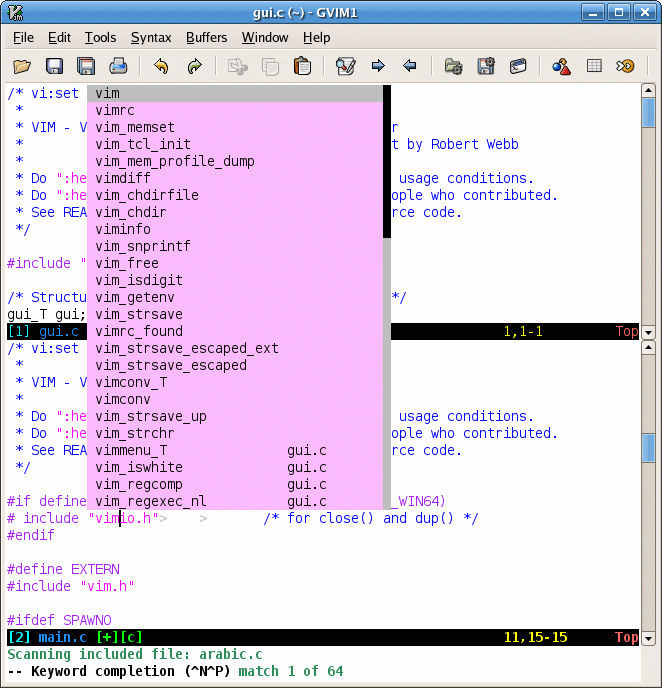
\includegraphics[scale=0.2]{vim}
\end{center}
\caption{Screenshot of GVim}
\end{figure}
}
\end{frame}


% vim history
% vim is a modal editor, command mode and insert mode
In this workshop, we will introduce you to the Vim editor.  Vim stands for Vi
IMproved, it is created by Bram Moolenaar (now working at Google) as an
improvement of an earlier editor called vi by Bill Joy (co-founder of Sun
Microsystems).  Vim is a modal editor. This means, depending on the current
mode, different keys have different effects (see Figure \ref{fig:vim_modes}).  
For example in Normal mode, pressing `x' key deletes the character under the
cursor, while in Insert mode, it adds the character `x' to the text file. This
allows Vim to use almost all the keys on your keyboard for issuing commands.  

\begin{frame}
\ftitle{Vim is a modal editor}
\begin{figure}
\begin{center}
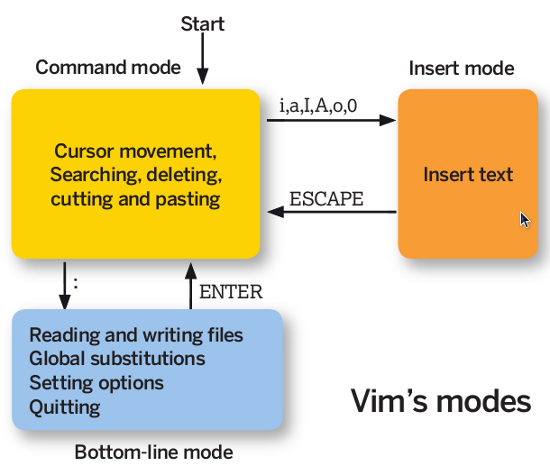
\includegraphics[scale=0.4]{vim_modes}
\end{center}
\caption{Different modes of Vim and how to switch between them}
\label{fig:vim_modes}
\end{figure}
\end{frame}

In the following activity, we will use Vim to create a simple text file. 

% ACTIVITY
\begin{frame}{Activity: Text editing with Vim}
\begin{enumerate}
\item From the Secure Shell Client window start Vim and create a new file using
the command \cmd{vim hello.txt}
\item Vim puts you in Normal mode by default. Switch to Insert mode using the
`i' key. \cmd{i} 
\item Type a short message to introduce yourself.
\item Now return to Normal mode by pressing the Escape key. \cmd{<Esc>} 
\item Save the file and exit Vim by pressing `ZZ' \cmd{ZZ}
\end{enumerate}
\end{frame}

\subsection{Organising your home directory}
Files on UNIX are arranged in a hierarchical structure, like an inverted tree
(see Figure \ref{fig:dir}).  The top of the hierarchy is traditionally called
root (written as a slash /)

\begin{frame}
\ftitle{UNIX Directory Tree}
\begin{figure}
\begin{center}
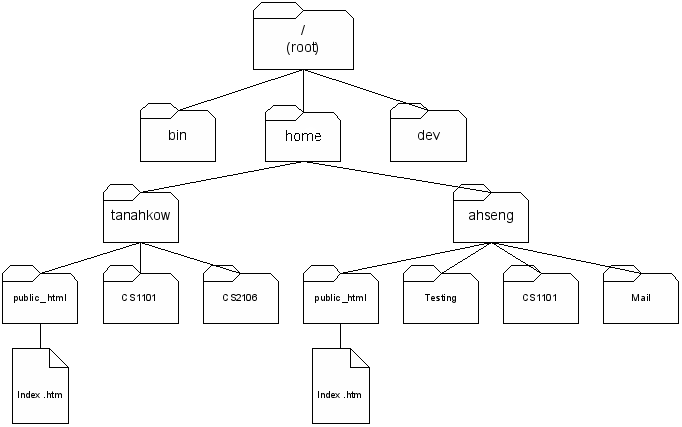
\includegraphics[scale=0.4]{file_home}
\end{center}
\caption{A subset of the UNIX directory tree showing home directories}
\label{fig:dir}
\end{figure}
\end{frame}

Directories allow you to organising your files on UNIX.  Certain directories
have special meaning in UNIX. For example, the contents of the directory named
\texttt{public\_html} in your home directory is interpreted by the web server as
your homepage at \url{http://www.comp.nus.edu.sg/~unix_username}

Sometimes you might want to share a file with your friends but it is too large
to send through email. You can make use of the 2Gb in your UNIX account to host
the file on your website. The following activity, shows you how to share a file
on your personal website.  

% ACTIVITY
\begin{frame}[allowframebreaks=0.6]{Activity: \texttt{sunfire} as a web host}
\begin{enumerate}
\item Find out your home directory using the following command
\cmd{pwd}
\item Create a directory under your home directory named
\texttt{public\_html}. \cmd{mkdir public\_html}
\item Move \texttt{hello.txt} into the \texttt{public\_html} directory. \cmd{mv hello.txt public\_html}
\item Change the permissions on \texttt{public\_html} so that it is readable by
the web server. \cmd{chmod a+rx public\_html}
\item Change your current directory to \texttt{public\_html}. \cmd{cd public\_html}
\item Change the permission on \texttt{hello.txt} so that it is readable by the
web server.  \cmd{chmod a+r hello.txt}
\item Ask the person next to you to download hello.txt from your personal
website at \url{http://www.comp.nus.edu.sg/~unix_username/hello.txt}
\end{enumerate}
\end{frame}


\subsection{Some useful applications on UNIX}
A major part of the operating system that the user interacts with are the
utilities that helps the user to perform everyday tasks such as editing files,
printing and reading email.     

You have already used a number of such utilities such as \texttt{mkdir} (make
directory), \texttt{mv} (move), \texttt{chmod} (change modifiers/permissions)
and \texttt{cd} (change directory).

In the next activity, you will learn a number of utilities related to printing.
There are a number of printers that are exclusive to SoC students, they are
located in COM1 level 1 and basement.  

% ACTIVITY: Printing
\begin{frame}{Activity: Printing}
\mode<presentation>{
\begin{figure}
\begin{center}
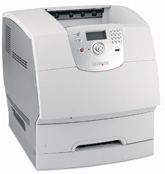
\includegraphics[scale=0.4]{printer}
\end{center}
\caption{Lexmark printers at COM1}
\end{figure}
}

\begin{itemize}
\item View the status of the print queue, use \texttt{lpq}, \cmd{lpq -P pstsc}
\item Remove a print job after it has been sent, use \texttt{lprm}, \cmd{lprm -P pstsc 89}
\item Check your print quota, use \texttt{pusage}, \cmd{pusage}
\end{itemize}

\end{frame}

UNIX utilities are simple focused programs operating using a common
communication protocol. This is summed up by Douglas McIlroy (inventor of UNIX
pipes) as the UNIX philosophy.   

% This is analogous to the way web services communicate
% analogy with Internet web services, assembly line

% ls
% man
% prog1 $|$ prog2
% prog $>$ file

% UNIX philosophy
\begin{frame}{The UNIX Philosophy}
\begin{quote}
Write programs that do one thing and do it well.

Write programs to work together.

Write programs to handle text streams, because that is a universal interface.
\end{quote}
\begin{flushright}
\mode<presentation>{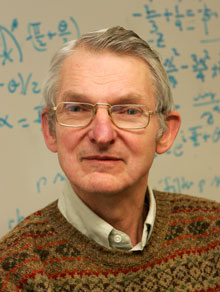
\includegraphics[height=0.3\textheight]{mcilroy}\\}
-- Douglas McIlroy
\end{flushright}
\end{frame}


We will see the UNIX philosophy in action in our next activity, which makes use
of three UNIX utility programs to analyse SMS messages.  

% ACTIVITY: SMS Word Count
\begin{frame}{Activity: SMS Word Count}
\mode<presentation>{
\begin{figure}
\begin{center}
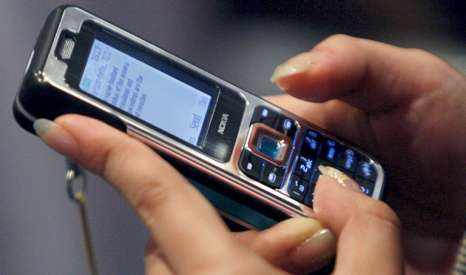
\includegraphics[scale=0.5]{sms}
\end{center}
\end{figure}
}
Your friend from FASS is studying SMS language as part of a course project. She
collected a number of SMS messages and would like to find out the frequency of
each word. 
\end{frame}

\begin{frame}[fragile]
\ftitle{Activity: SMS Word Count}
\begin{columns}
\begin{column}{0.5\textwidth}
For example, given the following text file:
\begin{verbatim}
U wan 2 haf lunch i'm in da 
canteen now.
Haf u found him? I feel so 
stupid da v cam was working.
Where r we meeting?
I went to ur hon lab but no 
one is there.
\end{verbatim}
\end{column}
\begin{column}{0.5\textwidth}
The desired output is:
\begin{verbatim}
      .
      .
      .
      1 we
      1 went
      1 Where
      1 working.
      2 da
      2 I
\end{verbatim}
\end{column}
\end{columns}
\end{frame}

% Hugo: Input file is too large, maybe reduce to 5 lines of SMS
% Hugo: introduce grep
% introduce man to find the option of sort and uniq to use

\begin{frame}[fragile]
\frametitle{Activity: \texttt{sort} and \texttt{uniq}}
Two UNIX utility programs are related to our task.  

\begin{block}{\texttt{sort}}
\begin{tabular}{c c c}
Input: & & Output: \\
dog    & & bat \\
bat    &$\longrightarrow$& cat \\
log    & & dog \\
cat    & & log \\
\end{tabular}
\end{block}

\begin{block}{\texttt{uniq}}
\begin{tabular}{c c c}
Input: & & Output: \\
dog    & & dog \\
dog    &$\longrightarrow$& cat \\
cat    & & dog \\
cat    & & cat \\
dog    & & \\
cat    & & \\
cat    & & \\
\end{tabular}
\end{block}
\end{frame}

\begin{frame}[allowframebreaks=0.6]{Activity: SMS Word Count}

\begin{enumerate}
\item Download the file containing sms messages from \url{http://www.comp.nus.edu.sg/~melvin/UWS/SMSwords.txt} using wget 
\cmd{wget \url{http://www.comp.nus.edu.sg/~melvin/UWS/SMSwords.txt}}  
\item Sort the file.  \cmd{sort SMSwords.txt} 
\item Sort and remove duplicates.   \cmd{sort SMSwords.txt | uniq} 
\item We need to use a particular option of \texttt{uniq} which counts the
number of duplicates, read the manual page for \texttt{uniq}. Press \texttt{q}
to leave the manual page.   \cmd{man uniq} 
\item Sort and count words, \cmd{sort SMSwords.txt | uniq -???} 
\item Sort by the frequency, so that more frequent words appear later, 
\cmd{sort SMSwords.txt | uniq -??? | sort -n}
\end{enumerate}
\end{frame}

If there is additional time during the workshop, you may wish to setup a
homepage which is accessible at \url{http://www.comp.nus.edu.sg/~unix_username}.
The details are provided in the following activity.  

% ACTIVITY: setting up index.html
\begin{frame}[fragile]
\frametitle{Activity: Setting up your homepage (Optional)}
Instead of using \texttt{hello.txt}, create a file named \texttt{index.html} and
put it in your \texttt{public\_html} directory. Remember to change its
permissions to readable by all.  

\begin{verbatim}
<html>
<head>
<title>Sample index page</title>
</head>
<body>
Hello World
</body>
</html>
\end{verbatim}
\end{frame}

\section{Summary}

\begin{frame}
\ftitle{Summary}
In this workshop, we have covered the following topics:
\begin{itemize}
\item UNIX from past to present
\item Connecting to \texttt{sunfire} via ssh
\item Text editing using Vim
\item Using \texttt{sunfire} as a web host
\item Manipulating text files using UNIX utilities
\end{itemize}
\end{frame}

Finally, after we are done with what we need to do in the UNIX environment, we
have to logout of the system.  

% ACTIVITY
\begin{frame}{Activity: Logging out of \texttt{sunfire}}
To log out of \texttt{sunfire}, use the \texttt{logout} command, \cmd{logout}
\end{frame}

\section{Resources}

\begin{frame}{Computing Resources in SoC}
\begin{itemize}
\item Description of facilities in SoC, \url{https://www.comp.nus.edu.sg/cf} and \url{https://mysoc.nus.edu.sg/~wiki}
\item Web based services, mySoC, \url{https://mysoc.nus.edu.sg}
\item SoC Webmail \url{https://mysoc.nus.edu.sg/~webmail}
\item SSH Secure Shell Client 3.2.9, \url{http://www.comp.nus.edu.sg/~cs1101x/2_resources/SSHSecureShellClient-3.2.9.exe}
\end{itemize}
\end{frame}

\end{document}
